\cotefile{90}
\scanpage{2}
% archive sheet number: 1

\figure{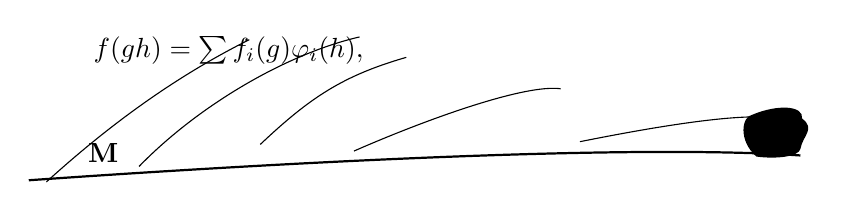
\begin{tikzpicture}[x=.70cm,y=.70cm]
\node[anchor=west] at (1,2.35) {$\deleted{f(gh)=\sum f_i(g)\varphi_i(h),}$};
\node[anchor=west] at (.9,.50) {\uline{$\mathbf M$}};
\draw[thick] (0,0) .. controls (5,.35) and (11,.65) .. (14,.45);
\draw (.32,-.03) .. controls (1.4,.95) and (2.6,1.85) .. (4,2.55);
\draw (2,.25) .. controls (3.1,1.38) and (4.7,2.3) .. (6,2.6);
\draw (4.2,.65) .. controls (5.1,1.5) and (5.7,1.9) .. (6.85,2.23);
\draw (5.9,.53) .. controls (7.2,1.1) and (9,1.75) .. (9.65,1.66);
\draw (10,.7) .. controls (11.2,.94) and (12.5,1.16) .. (13.25,1.15);
\fill (13.2,.43) .. controls (12.87,.72) and (12.93,1.16) .. (13.13,1.19) .. controls (13.58,1.38) and (14.06,1.36) .. (14.03,1.12) .. controls (14.28,.93) and (14.04,.81) .. (14,.57) .. controls (13.97,.43) and (13.57,.38) .. cycle;
\end{tikzpicture}}

\uline{Lemme 1} Soit $A$ un anneau de Dedekind \deleted{\unsure{qui n'est pas un corps}}, $M$ un $A$-module plat. \deleted{Conditions équivalentes} Pour $\forall$ sous-module $N$ de $M$, soit $\widetilde N$ l'image inverse dans $M$ du sous-module de Torsion de $M/N$. Donc $\widetilde N/N$ est un module de torsion.

Cond. équivalentes a) b) c) d)

a) $\forall\, N$ de type fini, $\widetilde N/N$ est de longueur finie, i.e. $\widetilde N$ est de t.f. \margin{$\unsure{\Updownarrow|\Uparrow}$}

b) \deleted{$A$ est un corps,} \inserted{Si $A$ n'est pas un corps,} Il n'existe pas de sous-module de $M$ isomorphe à \deleted{\unsure{$A_p$|$A(p)$}} \inserted{$A(p)=\bigcup_n p^{-n}=\Gamma(S-\{p\},\underline{O}_S)$ $(S=\operatorname{Spec} A)$,} $p$ est un idéal maximal de $A$ \deleted{\unsure{ou} $A$ est un corps.}

c) \deleted{\unsure{Pour tout}} \inserted{Si $A$ n'est pas un corps,} Pour \deleted{$\forall$} \deleted{\unsure{$p$}} idéal maximal $p$ de $A$, $M_p$ ne contient pas de $K$-module isom. à $K$. \margin{$\Updownarrow$}

d) $M=\underset{\longrightarrow}{\lim} M_i$, les $M_i\subset M$ \deleted{de type} fini et ``saturés'', i.e. \inserted{$M_i\unsure{-|\to}M_j$ \unsure{tels|dès} que $M_i$ facteur direct \unsure{de|dans} $M_j$.}

Pour que ces conditions soient \deleted{\unsure{satisfaites}}, il suffit que l'on ait :

e) les formes linéaires sur $M$ séparent, i.e.
\[
\underline M\hookrightarrow A^I \qquad (I\text{ un ensemble})
\]
[condition vérifiée si $M$ contenu \unsure{ds|dans} un libre, \deleted{\unsure{p.}} i.e. $M$ projectif]

C'est aussi nécessaire si $M$ a un ens. dénombrable de générateurs.
